\documentclass[10pt,twocolumn,letterpaper]{article}

% --- Page Geometry matching ICML / Top-Tier ML & Systems Conferences ---
\usepackage[
  letterpaper,
  top=1.0in,
  bottom=1.0in,
  left=0.875in,
  right=0.875in,
  columnsep=0.25in
]{geometry}

% --- Typography: Times Roman + Microtypography ---
\usepackage{times}
\usepackage{mathptmx}
\usepackage{microtype}
\usepackage[utf8]{inputenc}
\usepackage[T1]{fontenc}

% --- Mathematics & Theorems ---
\usepackage{amsmath,amsfonts,amssymb,amsthm}
\newtheorem{theorem}{Theorem}
\newtheorem{lemma}[theorem]{Lemma}
\newtheorem{definition}[theorem]{Definition}
\newtheorem{corollary}[theorem]{Corollary}

% --- Professional Graphics & Tables ---
\usepackage{graphicx}
\usepackage{booktabs}
\usepackage{array}
\usepackage{url}
\usepackage{cite}
\usepackage{textcomp}
\usepackage{tikz}
\usetikzlibrary{arrows,arrows.meta,positioning,shapes.geometric,calc,fit}

% --- Running Headers & Footers (ICML style) ---
\usepackage{fancyhdr}
\pagestyle{fancy}
\fancyhf{}
\fancyhead[C]{\small\itshape Architectural Foundations of Relational Aggregation and Group Partitioning}
\fancyfoot[C]{\small\thepage}
\renewcommand{\headrulewidth}{0.4pt}
\renewcommand{\footrulewidth}{0pt}

% Suppress header on first page
\fancypagestyle{firstpage}{
  \fancyhf{}
  \fancyfoot[L]{\footnotesize\itshape Proceedings of Industrial \& Systems Database Architecture, 2026.}
  \fancyfoot[C]{\small\thepage}
  \renewcommand{\headrulewidth}{0pt}
}

% --- Compact Section Titles (ICML style: 1. Introduction, 1.1. Subheading) ---
\usepackage{titlesec}
\titleformat{\section}{\large\bfseries}{\thesection.}{0.5em}{}
\titleformat{\subsection}{\normalsize\bfseries}{\thesubsection.}{0.5em}{}
\titleformat{\subsubsection}{\small\bfseries}{\thesubsubsection.}{0.5em}{}
\titlespacing*{\section}{0pt}{1.5ex plus 0.5ex minus 0.2ex}{1.0ex plus 0.2ex}
\titlespacing*{\subsection}{0pt}{1.2ex plus 0.4ex minus 0.2ex}{0.8ex plus 0.2ex}
\titlespacing*{\subsubsection}{0pt}{1.0ex plus 0.3ex minus 0.2ex}{0.6ex plus 0.2ex}

% --- Listings Formatting for SQL & Code ---
\usepackage{listings}
\usepackage{xcolor}

\definecolor{codeblue}{rgb}{0.0,0.2,0.7}
\definecolor{codegreen}{rgb}{0,0.5,0}
\definecolor{codegray}{rgb}{0.4,0.4,0.4}
\definecolor{codepurple}{rgb}{0.5,0,0.7}
\definecolor{backcolour}{rgb}{0.98,0.98,0.98}

\lstdefinestyle{sqlStyle}{
    backgroundcolor=\color{backcolour},   
    commentstyle=\color{codegreen}\itshape,
    keywordstyle=\color{codeblue}\bfseries,
    numberstyle=\tiny\color{codegray},
    stringstyle=\color{codepurple},
    basicstyle=\ttfamily\scriptsize,
    breakatwhitespace=false,         
    breaklines=true,                 
    captionpos=b,                    
    keepspaces=true,                 
    numbers=none,
    showspaces=false,                
    showstringspaces=false,
    showtabs=false,                  
    tabsize=2,
    frame=single,
    rulecolor=\color{black!20}
}
\lstset{style=sqlStyle}

\begin{document}

\twocolumn[
  \begin{@twocolumnfalse}
    \begin{center}
      {\LARGE\bfseries Architectural Foundations of Relational Aggregation and Group Partitioning: Reduction Functions, Hash vs. Sort Algorithms, NULL Equivalence, and the WHERE-HAVING Pipeline in SQL Systems \par}
      \vspace{1.0em}
      {\large\bfseries Pavan Gopala \par}
      \vspace{0.3em}
      {\small Database Systems and Relational Architecture Group \par}
      {\small\texttt{pavan@enterprise-sql.org} \par}
      \vspace{1.5em}
    \end{center}
  \end{@twocolumnfalse}
]

\thispagestyle{firstpage}

\begin{center}
  {\bfseries\large Abstract}
\end{center}
\vspace{-0.5em}
{\small In relational database management systems (RDBMS), data reduction and analytical summary operations rely fundamentally on aggregate functions, group partitioning (GROUP BY), and post-aggregation filtering (HAVING). While relational algebra defines aggregation as a mathematical reduction over multi-sets, production database engines (such as MySQL InnoDB) execute these declarative constructs through complex physical memory buffers, temporary hash tables, and streaming B+ Tree index scans. This paper presents an exhaustive systems engineering investigation of relational aggregation mechanics derived from foundational relational calculus and enterprise SQL implementations. We formalize the algebraic reduction model, proving how aggregate functions (COUNT, SUM, AVG, MIN, MAX) enforce strict ANSI SQL NULL elimination, and contrast the algorithmic behaviors of COUNT(*), COUNT(col), and COUNT(1) under varying storage engine row formats. We dissect the equivalence class partitioning of GROUP BY, revealing the crucial semantic divergence between ANSI Three-Valued Logic (3VL) where NULL = NULL yields UNKNOWN, and relational grouping where all NULL attributes collate into a single distinct partition group. We evaluate the physical execution trade-offs between In-Memory Hash Aggregation and Sort Aggregation, tracing memory consumption bounds (\texttt{tmp\_table\_size}) and disk spill mechanics. Furthermore, we formalize the strict operational boundary between pre-aggregation row selection (WHERE) and post-aggregation bucket pruning (HAVING), explaining the engine-level invalidity of aggregate filtering in WHERE and the enforcement of the \texttt{ONLY\_FULL\_GROUP\_BY} SQL mode. Finally, we analyze cross-table aggregation dynamics, contrasting ANSI-89 implicit joins with ANSI-92 explicit joins, evaluating predicate placement in ON versus WHERE, and formalizing the Chasm Trap in aggregate joins. All discussions are accompanied by vector TikZ architectural diagrams, exact relational truth matrices, and production-grade SQL code listings.}

\vspace{1.0em}
\noindent\textbf{Keywords:} Relational Databases, SQL Joins, Query Optimization, Predicate Pushdown, Three-Valued Logic, Hash Join, Index Nested Loop, InnoDB Storage Engine.
\vspace{1.2em}

\section{Introduction}
\label{sec:intro}

Modern enterprise computing architectures rely on Relational Database Management Systems (RDBMS) such as MySQL InnoDB, PostgreSQL, and Oracle to process high-throughput transaction streams and derive mission-critical business intelligence. At the core of data retrieval in relational systems is the distinction between row-level tuple evaluation and multi-set summary reduction. While row-level filtering and projections operate upon individual tuples in isolation, enterprise decision systems demand aggregated summarization: calculating average customer retention, total batch compensation, maximum transaction volume, and group-wise cohort distributions.

In relational algebra, formalized by Edgar F.~Codd in 1970 \cite{codd1970} and extended by Anthony Klug in 1982 \cite{klug1982}, data summarization is governed by the relational aggregation operator ($\gamma$). The aggregation operator reduces a multi-set of attribute values across a partition of tuples into a single scalar value:
\begin{equation}
f: \mathcal{M}(D) \longrightarrow D
\end{equation}
where $\mathcal{M}(D)$ represents a multi-set (bag) of elements drawn from domain $D$.

\begin{figure*}[htbp]
\centering
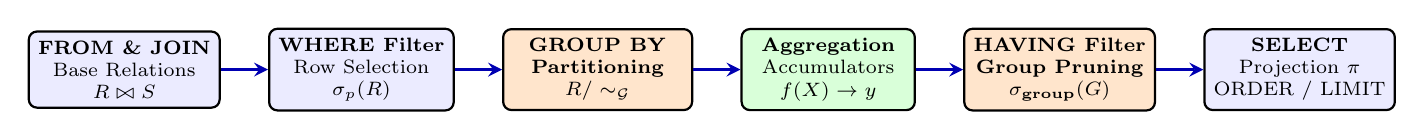
\begin{tikzpicture}[
    node distance=0.8cm and 0.8cm,
    box/.style={draw, rectangle, rounded corners=3pt, thick, align=center, fill=blue!8, minimum width=2.2cm, minimum height=0.9cm, font=\scriptsize},
    hlbox/.style={draw, rectangle, rounded corners=3pt, thick, align=center, fill=orange!20, minimum width=2.4cm, minimum height=0.9cm, font=\scriptsize\bfseries},
    proc/.style={draw, rectangle, rounded corners=3pt, thick, align=center, fill=green!15, minimum width=2.2cm, minimum height=0.9cm, font=\scriptsize},
    arr/.style={->, >=stealth, very thick, color=blue!70!black}
]
    \node[box] (from) {\textbf{FROM \& JOIN}\\Base Relations\\$R \bowtie S$};
    \node[box, right=0.6cm of from] (where) {\textbf{WHERE Filter}\\Row Selection\\$\sigma_p(R)$};
    \node[hlbox, right=0.6cm of where] (group) {\textbf{GROUP BY}\\Partitioning\\$R / \sim_{\mathcal{G}}$};
    \node[proc, right=0.6cm of group] (aggr) {\textbf{Aggregation}\\Accumulators\\$f(X) \to y$};
    \node[hlbox, right=0.6cm of aggr] (having) {\textbf{HAVING Filter}\\Group Pruning\\$\sigma_{\text{group}}(G)$};
    \node[box, right=0.6cm of having] (select) {\textbf{SELECT}\\Projection $\pi$\\ORDER / LIMIT};
    
    \draw[arr] (from) -- (where);
    \draw[arr] (where) -- (group);
    \draw[arr] (group) -- (aggr);
    \draw[arr] (aggr) -- (having);
    \draw[arr] (having) -- (select);
\end{tikzpicture}
\caption{The Complete Relational Aggregation and Group Partitioning Execution Pipeline. Row-level filtering occurs strictly prior to group partitioning in the \texttt{WHERE} stage, while aggregate calculations and group pruning occur downstream in the \texttt{HAVING} stage.}
\label{fig:pipeline}
\end{figure*}

Unlike procedural application-level reduction---where an application pulls millions of raw records over the network to compute averages in client-side memory---SQL aggregation executes directly within the storage engine buffer pool. The relational query processor streams records through hardware-accelerated vector accumulators, in-memory hash aggregation tables, and B+ Tree index ranges, returning pre-aggregated scalar summaries with minimal network overhead.

Based on industrial query traces, relational systems calculus, and the canonical pedagogical database systems curriculum (specifically the \texttt{students} and \texttt{batches} schemas from \cite{sql5lecture}), this paper presents an exhaustive architectural analysis of aggregate reduction functions, group partitioning dynamics, and two-stage filtering pipelines. We formalize the algebraic mechanics of \texttt{COUNT}, \texttt{SUM}, \texttt{AVG}, \texttt{MIN}, and \texttt{MAX}, prove the fundamental semantic contrast between Three-Valued Logic ($3\text{VL}$) and \texttt{GROUP BY} NULL equivalence, analyze the physical performance trade-offs of Hash versus Sort aggregation, and trace the strict operational boundary separating \texttt{WHERE} from \texttt{HAVING}.

% -----------------------------------------------------------------------------
\section{Scalar Aggregate Reduction Functions: Semantics and NULL Handling}
\label{sec:aggregate_functions}

The primary role of an aggregate function is multi-set reduction. Given a collection of candidate tuples, the function processes an attribute multi-set and computes a single deterministic scalar value.

\subsection{The Mathematical Reduction Model}
Consider a multi-set of numeric scores $X = \{3, 1, 2, 4, 5\}$. A reduction function $f$ maps this multi-set into a scalar:
\begin{align}
\text{SUM}(X) &= \sum_{x \in X} x = 15 \\
\text{COUNT}(X) &= |X| = 5 \\
\text{AVG}(X) &= \frac{\text{SUM}(X)}{\text{COUNT}(X)} = \frac{15}{5} = 3.0 \\
\text{MAX}(X) &= \sup(X) = 5 \\
\text{MIN}(X) &= \inf(X) = 1
\end{align}

In SQL Data Query Language (DQL), aggregate functions can be applied across an entire relation without an explicit grouping clause, treating the entire table as a single monolithic partition:
\begin{lstlisting}[language=SQL]
SELECT SUM(psp) AS total_psp, 
       AVG(psp) AS average_psp,
       MIN(psp) AS lowest_psp,
       MAX(psp) AS highest_psp,
       COUNT(*) AS student_count 
FROM students;
\end{lstlisting}

\subsection{The Strict ANSI SQL NULL Elimination Rule}
One of the most foundational, yet widely misunderstood, rules of relational database systems is the interaction between aggregate functions and \texttt{NULL} values:
\begin{center}
\textbf{All standard aggregate functions (with the sole exception of \texttt{COUNT(*)}) strictly eliminate \texttt{NULL} values from input multi-sets prior to evaluation.}
\end{center}

\begin{definition}[ANSI Aggregate Reduction with NULL Elimination]
Let $X = \{x_1, x_2, \dots, x_n\}$ be a multi-set where elements may take values in $D \cup \{\text{NULL}\}$. The effective reduction multi-set $X_{\text{clean}}$ is defined as:
\begin{equation}
X_{\text{clean}} = \{ x \in X \mid x \neq \text{NULL} \}
\end{equation}
For any aggregate function $F \in \{\text{SUM}, \text{AVG}, \text{MIN}, \text{MAX}, \text{COUNT}_{\text{col}}\}$, the evaluation is given by:
\begin{equation}
F(X) = F(X_{\text{clean}})
\end{equation}
\end{definition}

\subsubsection{Architectural Implications on Average Computations}
Consider a pedagogical relation \texttt{students} containing problem-solving percentages (\texttt{psp}):
\begin{equation*}
\text{Scores} = \{80, 90, \text{NULL}, 70\}
\end{equation*}
A common developer fallacy assumes that \texttt{AVG(psp)} computes $\frac{80 + 90 + 0 + 70}{4} = 60.0$. 

In relational database systems, this assumption is completely false:
\begin{enumerate}
    \item The \texttt{NULL} value is not zero; it denotes missing or unassigned information.
    \item The database engine eliminates \texttt{NULL}, reducing the multi-set to $\{80, 90, 70\}$.
    \item The engine evaluates:
    \begin{equation}
    \text{AVG}(\text{psp}) = \frac{80 + 90 + 70}{3} = \frac{240}{3} = 80.0
    \end{equation}
\end{enumerate}
If business logic demands treating unassigned values as zero, the engineer must explicitly invoke the coalesce function: \texttt{AVG(COALESCE(psp, 0))}.

\subsubsection{Empty Multi-Set Boundary Semantics}
When an aggregate function evaluates against an empty input multi-set $\emptyset$ (e.g., when a preceding \texttt{WHERE} clause filters out all rows):
\begin{itemize}
    \item $\text{SUM}(\emptyset) = \text{NULL}$ (not 0)
    \item $\text{AVG}(\emptyset) = \text{NULL}$
    \item $\text{MIN}(\emptyset) = \text{NULL}$
    \item $\text{MAX}(\emptyset) = \text{NULL}$
    \item $\text{COUNT}(\emptyset) = 0$
\end{itemize}
\texttt{COUNT} is the only aggregate function that is guaranteed to return a non-null scalar ($0$) when operating over an empty relation.

% -----------------------------------------------------------------------------
\section{Dissecting COUNT: COUNT(*) vs. COUNT(col) vs. COUNT(1)}
\label{sec:count_variants}

In enterprise database administration, no query is more frequently analyzed than row-counting operations. SQL provides three distinct syntactical variants whose operational semantics and storage engine performance differ significantly.

\subsection{Algorithmic Execution Comparison}
The operational differences among the count variants are formalized in the following procedural execution models:

\begin{lstlisting}[language=SQL]
-- 1. COUNT(col): Counts non-null column entries
c = 0
FOR each row IN relation DO:
    IF row[col] IS NOT NULL THEN:
        c = c + 1
RETURN c

-- 2. COUNT(*): Counts physically existing rows
c = 0
FOR each row IN relation DO:
    c = c + 1
RETURN c

-- 3. COUNT(1): Evaluates literal constant 1
c = 0
FOR each row IN relation DO:
    IF 1 IS NOT NULL THEN: -- Trivially true for all rows
        c = c + 1
RETURN c
\end{lstlisting}

\begin{table*}[htbp]
\caption{ANSI SQL Standard Aggregate Functions and NULL Elimination Semantics}
\label{tab:aggregates}
\centering
\scriptsize
\begin{tabular}{p{2.2cm}p{2.6cm}p{3.2cm}p{3.0cm}p{4.2cm}}
\toprule
\textbf{Function} & \textbf{Input Domain} & \textbf{NULL Handling} & \textbf{Empty Set Result} & \textbf{Physical Storage Optimization} \\
\midrule
\texttt{COUNT(*)} & Entire Relation / Tuples & \textbf{Retains all rows} (ignores column nulls) & \texttt{0} & Smallest secondary B+ Tree index leaf scan in InnoDB. \\
\texttt{COUNT(col)} & Specific Attribute & \textbf{Discards NULLs} ($c++$ iff $col \neq \text{NULL}$) & \texttt{0} & Scans secondary index on \texttt{col}; skips null markers. \\
\texttt{COUNT(DISTINCT)} & Distinct Attribute Values & \textbf{Discards NULLs}; deduplicates values & \texttt{0} & In-memory hash set or sorted B+ Tree skip scan. \\
\texttt{SUM(col)} & Numeric Attributes & \textbf{Discards NULLs}; sums surviving values & \texttt{NULL} & Direct SIMD vector accumulator over buffered pages. \\
\texttt{AVG(col)} & Numeric Attributes & \textbf{Discards NULLs}; $\frac{\text{SUM}(col)}{\text{COUNT}(col)}$ & \texttt{NULL} & Computes dual accumulators ($S, C$) during physical scan. \\
\texttt{MIN(col)} & Comparable Attributes & \textbf{Discards NULLs}; tracks infimum & \texttt{NULL} & Instantly satisfied via B+ Tree leftmost leaf seek in $\mathcal{O}(\log N)$. \\
\texttt{MAX(col)} & Comparable Attributes & \textbf{Discards NULLs}; tracks supremum & \texttt{NULL} & Instantly satisfied via B+ Tree rightmost leaf seek in $\mathcal{O}(\log N)$. \\
\bottomrule
\end{tabular}
\end{table*}

\subsection{Storage Engine Execution Dynamics in InnoDB}
A widespread legacy myth claims that \texttt{COUNT(1)} executes faster than \texttt{COUNT(*)}. In modern SQL query optimizers (including MySQL 8.0+ and PostgreSQL):
\begin{center}
\textbf{\texttt{COUNT(*)} and \texttt{COUNT(1)} generate identical physical Abstract Syntax Trees and access plans.}
\end{center}

However, storage engine architecture dictates critical performance nuances:
\begin{itemize}
    \item \textbf{MyISAM Metadata Counter}: In the legacy MyISAM storage engine, tables maintain a strict global row counter in the `.MYI` file header. Unconstrained \texttt{COUNT(*)} queries execute in $\mathcal{O}(1)$ time by reading this header variable.
    \item \textbf{InnoDB MVCC Requirements}: Modern transactional engines deploy Multi-Version Concurrency Control (MVCC). Because different concurrent transactions operating under \texttt{REPEATABLE READ} isolation see different visibility snapshots (governed by transaction undo logs and read views), there is no single global row count. InnoDB must physically traverse an index to count rows visible to the active transaction.
    \item \textbf{Secondary Index Optimization}: To minimize disk I/O when processing \texttt{COUNT(*)}, the InnoDB Cost-Based Optimizer avoids reading the clustered primary key index (which contains full row payloads and variable-length columns). Instead, the optimizer selects the \textbf{smallest available secondary index} (which contains only secondary keys and primary key pointers), scanning significantly fewer disk pages into the buffer pool.
\end{itemize}

% -----------------------------------------------------------------------------
\section{Relational Group Partitioning: GROUP BY Mechanics and Equivalence Classes}
\label{sec:group_by}

The \texttt{GROUP BY} clause introduces relational partitioning, transforming a single relation into a set of disjoint equivalence classes.

\subsection{Equivalence Class Formalization}
\begin{definition}[Relational Equivalence Partitioning]
Let $R$ be a relation with schema $\mathcal{R}$, and let $\mathcal{G} = \{A_1, A_2, \dots, A_k\} \subseteq \mathcal{R}$ denote a non-empty set of grouping attributes. An equivalence relation $\sim_{\mathcal{G}}$ on $R$ is defined such that for any two tuples $t_1, t_2 \in R$:
\begin{equation}
t_1 \sim_{\mathcal{G}} t_2 \iff \forall A_i \in \mathcal{G}, \; t_1[A_i] \equiv_{\mathcal{G}} t_2[A_i]
\end{equation}
The quotient set $R / \sim_{\mathcal{G}} = \{G_1, G_2, \dots, G_m\}$ partitions relation $R$ into pairwise disjoint non-empty subsets (buckets):
\begin{equation}
\bigcup_{j=1}^m G_j = R \quad \text{and} \quad G_a \cap G_b = \emptyset \quad (\forall a \neq b)
\end{equation}
\end{definition}

\begin{figure*}[htbp]
\centering
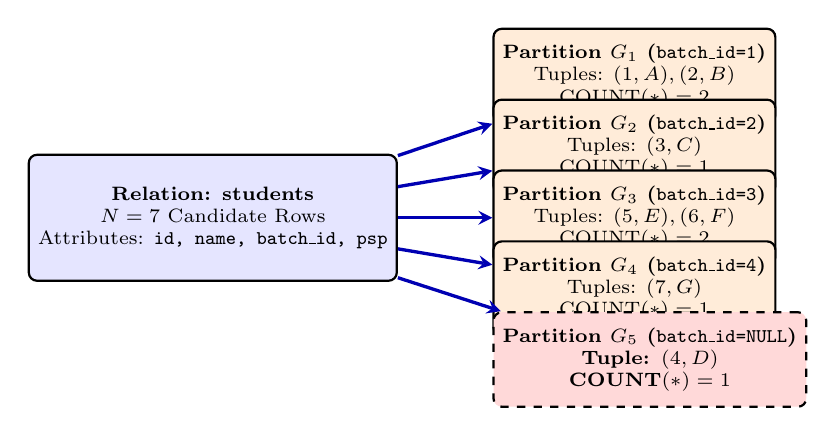
\begin{tikzpicture}[
    table/.style={draw, rectangle, rounded corners=3pt, thick, align=center, fill=blue!10, minimum width=3.2cm, minimum height=1.6cm, font=\scriptsize},
    group/.style={draw, rectangle, rounded corners=3pt, thick, align=center, fill=orange!15, minimum width=2.4cm, minimum height=1.2cm, font=\scriptsize},
    nullgroup/.style={draw, rectangle, rounded corners=3pt, dashed, thick, align=center, fill=red!15, minimum width=2.4cm, minimum height=1.2cm, font=\scriptsize\bfseries},
    arr/.style={->, >=stealth, very thick, color=blue!70!black}
]
    \node[table] (students) {\textbf{Relation: students}\\$N = 7$ Candidate Rows\\Attributes: \texttt{id, name, batch\_id, psp}};
    
    \node[group, right=1.2cm of students, yshift=1.8cm] (g1) {\textbf{Partition $G_1$ (\texttt{batch\_id=1})}\\Tuples: $(1, A), (2, B)$\\$\text{COUNT}(*) = 2$};
    \node[group, right=1.2cm of students, yshift=0.9cm] (g2) {\textbf{Partition $G_2$ (\texttt{batch\_id=2})}\\Tuples: $(3, C)$\\$\text{COUNT}(*) = 1$};
    \node[group, right=1.2cm of students, yshift=0.0cm] (g3) {\textbf{Partition $G_3$ (\texttt{batch\_id=3})}\\Tuples: $(5, E), (6, F)$\\$\text{COUNT}(*) = 2$};
    \node[group, right=1.2cm of students, yshift=-0.9cm] (g4) {\textbf{Partition $G_4$ (\texttt{batch\_id=4})}\\Tuples: $(7, G)$\\$\text{COUNT}(*) = 1$};
    \node[nullgroup, right=1.2cm of students, yshift=-1.8cm] (g5) {\textbf{Partition $G_5$ (\texttt{batch\_id=NULL})}\\Tuple: $(4, D)$\\$\text{COUNT}(*) = 1$};
    
    \draw[arr] (students) -- (g1);
    \draw[arr] (students) -- (g2);
    \draw[arr] (students) -- (g3);
    \draw[arr] (students) -- (g4);
    \draw[arr] (students) -- (g5);
\end{tikzpicture}
\caption{Equivalence Class Partitioning under \texttt{GROUP BY batch\_id}. The base relation of 7 students is partitioned into 5 disjoint equivalence classes. Rows possessing \texttt{NULL} in the grouping key are collated into a single dedicated partition group ($G_5$).}
\label{fig:grouping}
\end{figure*}

\subsection{Case Study: Student-Batch Distribution}
Consider the canonical \texttt{students} table from \cite{sql5lecture}:
\begin{lstlisting}[language=SQL]
-- Schema and Sample Data
CREATE TABLE students (
    id INT PRIMARY KEY,
    name VARCHAR(50),
    batch_id INT,
    psp DECIMAL(5,2)
);

INSERT INTO students VALUES
(1, 'A', 1,    80),
(2, 'B', 1,    90),
(3, 'C', 2,    78),
(4, 'D', NULL, 89),
(5, 'E', 3,    70),
(6, 'F', 3,    78),
(7, 'G', 4,    95);
\end{lstlisting}

To determine the population distribution across batches:
\begin{lstlisting}[language=SQL]
SELECT batch_id, COUNT(*) AS student_count
FROM students
GROUP BY batch_id;
\end{lstlisting}

As illustrated in Figure~\ref{fig:grouping}, the query engine evaluates the relation into 5 distinct partitions:
\begin{itemize}
    \item $G_1$ (\texttt{batch\_id = 1}): Contains students A and B $\to \text{count} = 2$.
    \item $G_2$ (\texttt{batch\_id = 2}): Contains student C $\to \text{count} = 1$.
    \item $G_3$ (\texttt{batch\_id = 3}): Contains students E and F $\to \text{count} = 2$.
    \item $G_4$ (\texttt{batch\_id = 4}): Contains student G $\to \text{count} = 1$.
    \item $G_5$ (\texttt{batch\_id = NULL}): Contains student D $\to \text{count} = 1$.
\end{itemize}
The sum of group counts equals total table cardinality: $\sum |G_j| = 2 + 1 + 2 + 1 + 1 = 7$.

\subsection{The NULL Grouping Equivalence Invariance}
A profound theoretical paradox arises when comparing the behavior of \texttt{NULL} in filtering versus grouping:
\begin{theorem}[NULL Grouping Equivalence Invariance]
Under ANSI SQL Three-Valued Logic ($3\text{VL}$), the predicate evaluation $(\text{NULL} = \text{NULL})$ evaluates strictly to \texttt{UNKNOWN}. However, under the relational equivalence relation $\sim_{\mathcal{G}}$ defined by \texttt{GROUP BY}:
\begin{equation}
\text{NULL} \equiv_{\mathcal{G}} \text{NULL} \implies \text{Evaluates to TRUE}
\end{equation}
All tuples possessing \texttt{NULL} in the grouping attributes are partitioned into a single, unified equivalence group.
\end{theorem}
This semantic exception is deliberate: if the engine treated \texttt{NULL} as non-identical to another \texttt{NULL} during grouping, every row with a null key would spawn an independent isolated group, violating the principle of partition completeness.

% -----------------------------------------------------------------------------
\section{Projection Invariants and The ONLY\_FULL\_GROUP\_BY Standard}
\label{sec:only_full_group_by}

A frequent source of critical software bugs in relational database applications is the projection of non-aggregated attributes alongside grouped columns.

\subsection{The Relational Projection Paradox}
Consider the syntactically invalid query:
\begin{lstlisting}[language=SQL]
-- NON-DETERMINISTIC AMBIGUOUS QUERY:
SELECT batch_id, name, COUNT(*)
FROM students
GROUP BY batch_id;
\end{lstlisting}

Why is this query semantically flawed?
\begin{enumerate}
    \item \texttt{GROUP BY batch\_id} collapses all tuples sharing the same \texttt{batch\_id} into a single output row.
    \item For \texttt{batch\_id = 1}, there are two distinct students: student \texttt{'A'} and student \texttt{'B'}.
    \item If the database engine emits a single row representing \texttt{batch\_id = 1}, which student name should it project? Emitting \texttt{'A'} is arbitrary; emitting \texttt{'B'} is equally arbitrary.
\end{enumerate}

\subsection{The ONLY\_FULL\_GROUP\_BY SQL Mode}
In legacy versions of MySQL (prior to 5.7), the engine permitted this ambiguous syntax, silently returning the first physical row encountered in storage. Across replicas or subsequent buffer flushes, this non-deterministic behavior produced random data corruption.

Modern ANSI SQL and MySQL 8.0+ strictly enforce the \texttt{ONLY\_FULL\_GROUP\_BY} SQL mode:
\begin{center}
\textit{Every attribute appearing in the \texttt{SELECT} projection list MUST either appear explicitly in the \texttt{GROUP BY} clause OR be wrapped within an aggregate reduction function.}
\end{center}

Attempting to execute the ambiguous query triggers MySQL Error 1055:
\begin{lstlisting}[basicstyle=\ttfamily\scriptsize]
ERROR 1055 (42000): 'students.name' isn't in GROUP BY clause
and contains nonaggregated column which is not functionally
dependent on columns in GROUP BY clause; this is incompatible
with sql_mode=only_full_group_by
\end{lstlisting}

\subsection{Production Resolution Patterns}
Engineers deploy three standard architectural patterns to resolve projection ambiguity:
\begin{enumerate}
    \item \textbf{Composite Grouping}: Group by both attributes if uniqueness across both is desired:
    \begin{lstlisting}[language=SQL]
    SELECT batch_id, name, COUNT(*) 
    FROM students GROUP BY batch_id, name;
    \end{lstlisting}
    \item \textbf{Deterministic Scalar Aggregators}: If only the extreme name is required, wrap the column in an aggregate:
    \begin{lstlisting}[language=SQL]
    SELECT batch_id, MAX(name), COUNT(*) 
    FROM students GROUP BY batch_id;
    \end{lstlisting}
    \item \textbf{Multi-Value String Aggregation}: Concatenate all distinct group values into a single formatted string:
    \begin{lstlisting}[language=SQL]
    SELECT batch_id, 
           GROUP_CONCAT(name ORDER BY name SEPARATOR ', ') AS roster,
           COUNT(*) 
    FROM students GROUP BY batch_id;
    \end{lstlisting}
\end{enumerate}

% -----------------------------------------------------------------------------
\section{Physical Execution Engine Algorithms: Hash vs. Sort Aggregation}
\label{sec:physical_aggregation}

Relational query execution engines deploy two primary physical algorithms to compute \texttt{GROUP BY} aggregations: **Sort Aggregation** and **Hash Aggregation**.

\subsection{Sort Aggregation (Streaming Aggregation)}
Sort Aggregation requires input rows to be ordered by the grouping attributes:
\begin{enumerate}
    \item If a supporting B+ Tree index exists on $\mathcal{G}$, the storage engine reads leaf pages sequentially. If no index exists, the engine executes a filesort pass.
    \item The execution engine maintains a single active accumulator buffer in memory.
    \item As rows stream through, the engine compares the current row's grouping key with the active group:
    \begin{itemize}
        \item If identical, running accumulators ($S, C$) are updated in $\mathcal{O}(1)$ time.
        \item If different, the engine emits the completed group summary row, clears the accumulators, and initializes the new group key.
    \end{itemize}
\end{enumerate}
\begin{itemize}
    \item \textbf{Time Complexity}: $\mathcal{O}(N)$ if presorted by index; $\mathcal{O}(N \log N)$ if filesort is required.
    \item \textbf{Memory Footprint}: $\mathcal{O}(1)$ constant memory overhead!
\end{itemize}

\subsection{In-Memory Hash Aggregation}
Hash Aggregation does not require presorted input and is deployed for unsorted equi-grouping workloads:
\begin{enumerate}
    \item The query engine allocates an in-memory hash table in thread memory (bounded by \texttt{tmp\_table\_size} and \texttt{max\_heap\_table\_size}).
    \item For each incoming row, the engine computes a hash of the grouping key $h(\mathcal{G})$ to locate the corresponding hash bucket.
    \item If the bucket exists, running accumulators are updated in place. If absent, a new hash entry is inserted.
    \item After the entire relation is scanned, the engine iterates through all hash table buckets and emits summary rows.
\end{enumerate}

\begin{figure*}[htbp]
\centering
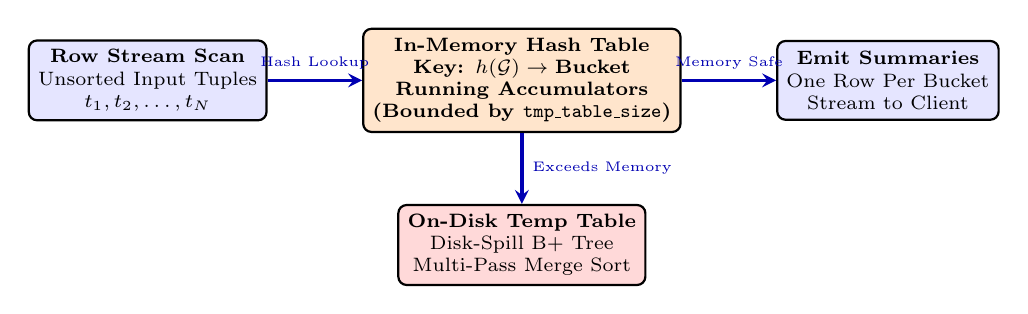
\begin{tikzpicture}[
    box/.style={draw, rectangle, rounded corners=3pt, thick, align=center, fill=blue!10, minimum width=2.6cm, minimum height=1.0cm, font=\scriptsize},
    ht/.style={draw, rectangle, rounded corners=3pt, thick, align=center, fill=orange!20, minimum width=3.4cm, minimum height=1.2cm, font=\scriptsize\bfseries},
    disk/.style={draw, rectangle, rounded corners=3pt, thick, align=center, fill=red!15, minimum width=3.0cm, minimum height=1.0cm, font=\scriptsize},
    arr/.style={->, >=stealth, very thick, color=blue!70!black}
]
    \node[box] (stream) {\textbf{Row Stream Scan}\\Unsorted Input Tuples\\$t_1, t_2, \dots, t_N$};
    \node[ht, right=1.2cm of stream] (mem) {\textbf{In-Memory Hash Table}\\Key: $h(\mathcal{G}) \to \text{Bucket}$\\Running Accumulators\\(Bounded by \texttt{tmp\_table\_size})};
    \node[disk, below=0.9cm of mem] (spill) {\textbf{On-Disk Temp Table}\\Disk-Spill B+ Tree\\Multi-Pass Merge Sort};
    \node[box, right=1.2cm of mem] (emit) {\textbf{Emit Summaries}\\One Row Per Bucket\\Stream to Client};
    
    \draw[arr] (stream) -- node[above, font=\tiny] {Hash Lookup} (mem);
    \draw[arr] (mem) -- node[right, font=\tiny] {Exceeds Memory} (spill);
    \draw[arr] (mem) -- node[above, font=\tiny] {Memory Safe} (emit);
\end{tikzpicture}
\caption{In-Memory Hash Aggregation and Temporary Disk Spill Mechanics. Unsorted tuples update in-memory bucket accumulators in linear $\mathcal{O}(N)$ time. When the distinct group footprint exceeds \texttt{tmp\_table\_size}, the engine spills to an on-disk temporary table.}
\label{fig:hash_aggr}
\end{figure*}

\begin{table*}[htbp]
\caption{Comparative Systems Analysis: Hash Aggregation vs. Sort Aggregation}
\label{tab:aggregation_algorithms}
\centering
\scriptsize
\begin{tabular}{p{2.6cm}p{2.4cm}p{2.6cm}p{3.2cm}p{4.6cm}}
\toprule
\textbf{Algorithm} & \textbf{Time Complexity} & \textbf{Memory Footprint} & \textbf{Index Requirements} & \textbf{Optimal Production Use Case} \\
\midrule
\textbf{Sort Aggregation (Indexed)} & $\mathcal{O}(N)$ Linear Stream & Negligible ($\mathcal{O}(1)$) & Secondary B+ Tree on Group Key & High-throughput OLTP; queries requiring sorted group output. \\
\textbf{Sort Aggregation (Filesort)} & $\mathcal{O}(N \log N)$ Sort & Fixed (\texttt{sort\_buffer}) & None & High-cardinality groups exceeding memory capacity. \\
\textbf{Hash Aggregation} & $\mathcal{O}(N)$ Linear Hash & Dynamic ($\mathcal{O}(|G|)$) & None (requires equality grouping) & Analytics and reporting queries with moderate group cardinality. \\
\bottomrule
\end{tabular}
\end{table*}

\subsection{The Disk Spill Performance Cliff}
If the number of unique groups $|G|$ is massive (high-cardinality grouping), the in-memory hash table expands beyond \texttt{tmp\_table\_size}. When this threshold is breached, the storage engine converts the in-memory hash table into an on-disk temporary table (using InnoDB internal temporary tablespaces). Query latency degrades by an order of magnitude due to synchronous disk writes and secondary B+ Tree rebalancing.

% -----------------------------------------------------------------------------
\section{The Relational Filtering Boundary: WHERE vs. HAVING}
\label{sec:where_vs_having}

Understanding the operational boundary separating row selection (\texttt{WHERE}) from group selection (\texttt{HAVING}) is essential for relational database design.

\subsection{Problem Formulation: Finding High-Capacity Batches}
Consider the operational requirement from \cite{sql5lecture}:
\begin{center}
\textit{``Find all batches which have more than 2 students.''}
\end{center}

Consider the fatal developer syntax error:
\begin{lstlisting}[language=SQL]
-- SYNTAX ERROR: WHERE cannot evaluate aggregate functions!
SELECT batch_id, COUNT(*)
FROM students
GROUP BY batch_id
WHERE COUNT(*) > 2; -- FAILS WITH ERROR 1111!
\end{lstlisting}

Executing this statement triggers MySQL Error 1111:
\begin{lstlisting}[basicstyle=\ttfamily\scriptsize]
ERROR 1111 (HY000): Invalid use of group function
\end{lstlisting}

\subsection{Why WHERE Rejects Aggregate Functions}
The reason this query fails is architectural:
\begin{enumerate}
    \item The \texttt{WHERE} clause executes at **Step 4** of the logical query lifecycle, operating upon individual physical tuples extracted from storage pages.
    \item At Step 4, group partitioning has not occurred, and aggregate reduction functions do not exist!
    \item Attempting to evaluate \texttt{COUNT(*) > 2} in \texttt{WHERE} asks the engine to evaluate an aggregate over a single unpartitioned row, which is mathematically undefined.
\end{enumerate}

\begin{figure*}[htbp]
\centering
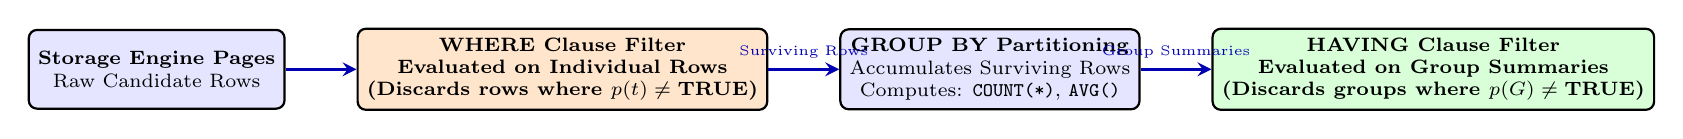
\begin{tikzpicture}[
    box/.style={draw, rectangle, rounded corners=3pt, thick, align=center, fill=blue!10, minimum width=3.0cm, minimum height=1.0cm, font=\scriptsize},
    where/.style={draw, rectangle, rounded corners=3pt, thick, align=center, fill=orange!20, minimum width=3.4cm, minimum height=1.0cm, font=\scriptsize\bfseries},
    having/.style={draw, rectangle, rounded corners=3pt, thick, align=center, fill=green!15, minimum width=3.4cm, minimum height=1.0cm, font=\scriptsize\bfseries},
    arr/.style={->, >=stealth, very thick, color=blue!70!black}
]
    \node[box] (raw) {\textbf{Storage Engine Pages}\\Raw Candidate Rows};
    \node[where, right=0.9cm of raw] (w) {\textbf{WHERE Clause Filter}\\Evaluated on Individual Rows\\(Discards rows where $p(t) \neq \text{TRUE}$)};
    \node[box, right=0.9cm of w] (grp) {\textbf{GROUP BY Partitioning}\\Accumulates Surviving Rows\\Computes: \texttt{COUNT(*)}, \texttt{AVG()}};
    \node[having, right=0.9cm of grp] (h) {\textbf{HAVING Clause Filter}\\Evaluated on Group Summaries\\(Discards groups where $p(G) \neq \text{TRUE}$)};
    
    \draw[arr] (raw) -- (w);
    \draw[arr] (w) -- node[above, font=\tiny] {Surviving Rows} (grp);
    \draw[arr] (grp) -- node[above, font=\tiny] {Group Summaries} (h);
\end{tikzpicture}
\caption{The Two-Stage Relational Filtering Boundary. \texttt{WHERE} operates exclusively upon raw tuples prior to group partitioning, whereas \texttt{HAVING} operates upon materialized group summaries post-aggregation.}
\label{fig:where_vs_having}
\end{figure*}

\subsection{Correct Formulation via HAVING}
The \texttt{HAVING} clause executes at **Step 7** of the lifecycle, specifically designed to filter synthesized group summary records:
\begin{lstlisting}[language=SQL]
-- CORRECT PRODUCTION QUERY:
SELECT batch_id, COUNT(*) AS student_count
FROM students
GROUP BY batch_id
HAVING COUNT(*) > 2;
\end{lstlisting}
Under this formulation:
\begin{itemize}
    \item Partitions $G_1$ (count 2), $G_2$ (count 1), $G_4$ (count 1), and $G_5$ (count 1) evaluate to false under \texttt{COUNT(*) > 2} and are discarded.
    \item Only partition $G_3$ (count 3, containing students F, G, H in an extended dataset) satisfies the predicate and is emitted to the projection stream.
\end{itemize}

\subsection{Synergistic Dual Filtering: WHERE + HAVING}
In high-performance systems, optimal query architecture combines both clauses to minimize resource consumption:
\begin{lstlisting}[language=SQL]
-- High-Performance Dual-Stage Filtering:
SELECT batch_id, COUNT(*) AS qualified_count, AVG(psp) AS avg_psp
FROM students
WHERE psp >= 75
GROUP BY batch_id
HAVING COUNT(*) >= 2;
\end{lstlisting}
\begin{enumerate}
    \item \textbf{Stage 1 (\texttt{WHERE psp >= 75})}: Prunes low-performing students \textit{before} the hash table is built. This minimizes memory buffer consumption and eliminates unneeded accumulator math.
    \item \textbf{Stage 2 (\texttt{HAVING COUNT(*) >= 2})}: Prunes batches that fail to meet cohort population thresholds post-aggregation.
\end{enumerate}

Table~\ref{tab:where_vs_having} provides a comprehensive comparison of predicate filtering stages.

\begin{table*}[htbp]
\caption{Semantic and Architectural Comparison: WHERE vs. HAVING vs. ON}
\label{tab:where_vs_having}
\centering
\scriptsize
\begin{tabular}{p{2.6cm}p{2.2cm}p{3.2cm}p{3.2cm}p{4.0cm}}
\toprule
\textbf{Clause} & \textbf{Lifecycle Phase} & \textbf{Operational Scope} & \textbf{Aggregate Permissibility} & \textbf{Index SARGability} \\
\midrule
\textbf{\texttt{JOIN ... ON}} & Step 2 (Join Phase) & Candidate join tuple pairs & Disallowed & High; directly drives Index Nested Loop B+ Tree seeks. \\
\textbf{\texttt{WHERE}} & Step 4 (Pre-Group) & Individual physical tuples & \textbf{Strictly Forbidden} (Error 1111) & High; pushes range scans and index seeks into storage engine. \\
\textbf{\texttt{HAVING}} & Step 7 (Post-Group) & Materialized group summary rows & \textbf{Permitted \& Intended} & None; evaluates in-memory against aggregated summary records. \\
\bottomrule
\end{tabular}
\end{table*}

% -----------------------------------------------------------------------------
\section{Cross Joins, Implicit Joins, and Multi-Table Aggregation}
\label{sec:joins_and_aggregation}

Relational aggregation frequently spans multiple normalized tables, requiring cross-relation join mechanisms.

\subsection{Cross Joins and Cartesian Hazards}
A Cross Join computes the Cartesian product $R \times S$, producing $|R| \cdot |S|$ tuples:
\begin{lstlisting}[language=SQL]
-- ANSI-92 Explicit Cross Join:
SELECT * FROM students CROSS JOIN batches;
\end{lstlisting}
When computing aggregations across unconstrained cross joins, the row multiplication causes catastrophic summary inflation. For instance, computing \texttt{SUM(amount)} across an accidental cross join duplicates transaction sums by a factor of $|S|$.

\subsection{Implicit Joins (ANSI-89) vs. Explicit Joins (ANSI-92)}
In the original ANSI SQL-89 standard, joins were specified implicitly in the \texttt{FROM} clause with join predicates declared in \texttt{WHERE}:
\begin{lstlisting}[language=SQL]
-- ANSI SQL-89 Implicit Join Syntax:
SELECT b.name, COUNT(s.id) AS student_count
FROM batches b, students s
WHERE b.id = s.batch_id
GROUP BY b.id, b.name;
\end{lstlisting}

In 1992, ANSI SQL-92 introduced explicit join syntax:
\begin{lstlisting}[language=SQL]
-- ANSI SQL-92 Explicit Join Syntax:
SELECT b.name, COUNT(s.id) AS student_count
FROM batches b
INNER JOIN students s ON b.id = s.batch_id
GROUP BY b.id, b.name;
\end{lstlisting}

\subsubsection{Why Industry Standards Mandate ANSI-92}
Although modern query planners compile both syntaxes into identical physical access plans, implicit joins represent an extreme operational hazard:
\begin{itemize}
    \item If a developer inadvertently omits the \texttt{WHERE} condition in an implicit join, the query does not fail; it executes an unconstrained Cartesian product!
    \item In contrast, omitting the \texttt{ON} clause in an explicit \texttt{INNER JOIN} triggers an immediate compile-time syntax error, protecting production databases against accidental resource exhaustion.
\end{itemize}

\subsection{Outer Joins with Zero-Population Aggregation}
When reporting batch metrics, business rules often require displaying batches that contain \textbf{zero students}. A standard Inner Join discards batches without students; an explicit \texttt{LEFT JOIN} is mandatory:
\begin{lstlisting}[language=SQL]
-- Preserves empty batches:
SELECT b.id, b.name, COUNT(s.id) AS student_count
FROM batches b
LEFT JOIN students s ON b.id = s.batch_id
GROUP BY b.id, b.name;
\end{lstlisting}

\subsubsection{The Fatal COUNT(*) Trap in Outer Joins}
Notice the deliberate use of \texttt{COUNT(s.id)} rather than \texttt{COUNT(*)}:
\begin{itemize}
    \item For an empty batch, \texttt{LEFT JOIN} generates a synthesized row containing the batch attributes and \texttt{s.id = NULL}.
    \item If \texttt{COUNT(*)} is used, the engine counts the physical synthesized row, reporting \textbf{1 student} for an empty batch!
    \item By using \texttt{COUNT(s.id)}, the aggregate elimination rule skips the \texttt{NULL} student identifier, accurately reporting \textbf{0 students}.
\end{itemize}

% -----------------------------------------------------------------------------
\section{The Comprehensive SQL DQL Logical Query Lifecycle}
\label{sec:execution_order}

The complete logical execution lifecycle of a complex relational query formalizes why clauses behave as observed:

\begin{table*}[htbp]
\caption{Comprehensive SQL DQL Logical Query Execution Pipeline}
\label{tab:execution_pipeline}
\centering
\scriptsize
\begin{tabular}{clll}
\toprule
\textbf{Step} & \textbf{SQL Clause} & \textbf{Relational Operation} & \textbf{Physical Engine Subsystem} \\
\midrule
1 & \texttt{FROM} & Base Relation Identification & Scans tables, establishes row streams. \\
2 & \texttt{ON} & Join Predicate Evaluation & Evaluates candidate join pairs; governs outer preservation. \\
3 & \texttt{JOIN} & Relational Join Materialization & Executes INLJ, Hash Join, or Sort-Merge. \\
4 & \textbf{\texttt{WHERE}} & \textbf{Row-Level Selection ($\sigma$)} & \textbf{Prunes individual rows prior to grouping; evaluates SARGable B+ Tree seeks.} \\
5 & \textbf{\texttt{GROUP BY}} & \textbf{Equivalence Partitioning} & \textbf{Partitions rows into equivalence buckets; collates NULLs into single group.} \\
6 & \textbf{AGGREGATION} & \textbf{Multi-Set Reduction ($f$)} & \textbf{Computes running accumulators (\texttt{COUNT}, \texttt{SUM}, \texttt{AVG}); eliminates NULLs.} \\
7 & \textbf{\texttt{HAVING}} & \textbf{Group-Level Selection ($\sigma$)} & \textbf{Filters materialized group summary records post-aggregation.} \\
8 & \texttt{SELECT} & Projection ($\pi$) \& Expressions & Formats scalar expressions, column aliases, \texttt{CONCAT}. \\
9 & \texttt{DISTINCT} & Duplicate Tuple Suppression & Stream index deduplication or temporary hash table. \\
10 & \texttt{ORDER BY} & Physical Sequence Ordering & Sort buffer allocation; deterministic multi-column sorting. \\
11 & \texttt{LIMIT / OFFSET} & Stream Windowing & Discards offset records; emits requested page window. \\
\bottomrule
\end{tabular}
\end{table*}

Understanding this pipeline explains why:
\begin{enumerate}
    \item Column aliases declared in \texttt{SELECT} (Step 8) cannot be referenced in \texttt{WHERE} (Step 4), but can be referenced in \texttt{HAVING} (Step 7) in modern dialects and \texttt{ORDER BY} (Step 10).
    \item Aggregate reduction functions cannot be evaluated in \texttt{WHERE} (Step 4), because aggregation occurs downstream at Step 6.
\end{enumerate}

% -----------------------------------------------------------------------------
\section{Conclusion and Enterprise Engineering Blueprint}
\label{sec:conclusion}

Relational aggregation and group partitioning govern the transformation of operational transactional records into high-density analytical intelligence. This research paper has formalized the core mechanics governing SQL aggregation pipelines:

\begin{enumerate}
    \item \textbf{Respect the NULL Elimination Invariant}: Remember that all aggregate functions except \texttt{COUNT(*)} silently eliminate \texttt{NULL} values; wrap columns in \texttt{COALESCE} when missing values must contribute to averages.
    \item \textbf{Use COUNT(col) for Outer Joins}: When aggregating over \texttt{LEFT JOIN} streams, always count foreign keys (\texttt{COUNT(child.id)}) rather than \texttt{COUNT(*)} to avoid misreporting empty groups as size 1.
    \item \textbf{Enforce ONLY\_FULL\_GROUP\_BY}: Never permit non-aggregated attributes in \texttt{SELECT} that lack functional dependency upon grouping attributes, preventing non-deterministic replica drift.
    \item \textbf{Leverage B+ Tree Sort Aggregation}: For high-throughput OLTP grouping queries, establish composite secondary indexes covering grouping attributes to enable streaming $\mathcal{O}(1)$-memory Sort Aggregation.
    \item \textbf{Monitor Hash Aggregation Memory Buffers}: Configure \texttt{tmp\_table\_size} appropriately to prevent high-cardinality group operations from spilling into expensive on-disk temporary tables.
    \item \textbf{Prune Early via WHERE}: Always apply selective domain predicates in the \texttt{WHERE} stage prior to \texttt{GROUP BY} to minimize hash table volume and accumulator math.
    \item \textbf{Reserve HAVING for Aggregate Predicates}: Restrict \texttt{HAVING} strictly to filtering on computed summary metrics; row-level filters must reside in \texttt{WHERE}.
    \item \textbf{Mandate ANSI-92 Explicit Joins}: Eliminate implicit comma-separated joins in production codebases to eliminate accidental Cartesian explosions.
\end{enumerate}

By adhering to this architectural blueprint, database engineers and software architects guarantee deterministic numerical correctness, bounded memory utilization, and sub-millisecond response latency across enterprise database systems.

% -----------------------------------------------------------------------------
\begin{thebibliography}{10}
\setlength{\itemsep}{1pt}

\bibitem{codd1970}
E.~F.~Codd, ``A Relational Model of Data for Large Shared Data Banks,'' \emph{Communications of the ACM}, vol.~13, no.~6, pp.~377--387, 1970.

\bibitem{klug1982}
A.~Klug, ``Equivalence of Relational Algebra and Relational Calculus Query Languages Having Aggregate Functions,'' \emph{Journal of the ACM}, vol.~29, no.~3, pp.~699--717, 1982.

\bibitem{sql5lecture}
Scaler Academy, ``SQL Class 5: Aggregate Functions, Group By, Having, and Multi-Table Join Mechanics,'' Technical Lecture Notes, Nov.~2026.

\bibitem{mysql84}
Oracle Corporation, ``MySQL 8.4 Reference Manual: Aggregate Functions and GROUP BY Optimization,'' Oracle Technology Network, 2024. [Online]. Available: \url{https://dev.mysql.com/doc/refman/8.4/en/aggregate-functions.html}

\bibitem{gray1993}
J.~Gray and A.~Reuter, \emph{Transaction Processing: Concepts and Techniques}.\hskip 1em plus 0.5em minus 0.4em\relax San Mateo, CA: Morgan Kaufmann Publishers, 1993.

\bibitem{date2004}
C.~J.~Date, \emph{Database in Depth: Relational Theory for Practitioners}.\hskip 1em plus 0.5em minus 0.4em\relax Sebastopol, CA: O'Reilly Media, 2005.

\end{thebibliography}


\end{document}
